\section{Results}

This section reports the empirical evidence generated by the executable pipeline and answers the three research questions directly. Its purpose is not only to present metric values, but also to show how the evidence should be read under the protocol defined in Methodology and Experimental Design. Throughout the section, the interpretation contract is preserved: policy and fairness quantities are reported as \textit{model-implied simulated regime contrasts}, not as observationally identified intervention effects.

The section follows the same logical progression as the framework itself. It begins with a figure-reading guide and direct answers to the research questions, then presents evidence for RQ1 (hazard quality), establishes the censoring-valid horizons required for interpreting downstream results, reports policy contrasts for RQ2, examines benchmark and robustness evidence, and finally reports subgroup results for RQ3. By the end of the section, the reader should expect a complete empirical answer to the paper objective: whether the framework can translate weekly risk into auditable policy and subgroup diagnostics under explicit reporting rules.

\subsection{How to Read the Figures in This Section}

To avoid ambiguous interpretation, each figure is tied to one research question, one metric family, and one reading rule. Table~\ref{tab:fig_reading_guide} summarizes that mapping and should be read as the figure-level evidence contract for this section.

\begin{table}[!t]
\centering
\scriptsize
\renewcommand{\arraystretch}{1.05}
\caption{Figure reading guide used in Results.}
\label{tab:fig_reading_guide}
\begin{tabular}{@{}>{\raggedright\arraybackslash}p{0.24\columnwidth}
                >{\raggedright\arraybackslash}p{0.24\columnwidth}
                >{\raggedright\arraybackslash}p{0.42\columnwidth}@{}}
\hline
Figure & What it answers & How to read it \\
\hline
Calibration reliability test &
RQ1 hazard quality &
Curves close to the diagonal indicate calibrated weekly risk. \\

Policy survival by week &
Temporal risk window (RQ1--RQ2 bridge) &
Compare slopes and separation near $T_{policy}$, $T_{eval\_metrics}$, and raw-support tail $T_{eval\_policy}$. \\

Censoring survival $G(t)$ &
Horizon validity under censoring &
Identify where $G(t)$ drops below $g_{min}=0.05$. \\

Policy $\Delta S(t)$ by week &
RQ2 policy contrast &
Positive $\Delta S(t)$ means policy survival exceeds baseline survival. \\

Benchmark dual-panel AUC &
Family robustness &
Check directional consistency across model families. \\

RQ3 gap at $T_{policy}$ and $T_{eval\_metrics}$ &
RQ3 subgroup contrast &
Read the sign and uncertainty of $\Delta Gap(T)$ at $T_{policy}$ and $T_{eval\_metrics}$. \\
\hline
\end{tabular}
\end{table}

\subsection{Direct Answers to the Research Questions}
\label{subsec:direct_answers}

Table~\ref{tab:rq_answers} gives the direct empirical answers before the detailed evidence is unpacked. The remainder of the section then substantiates each answer with figures, tables, and horizon-specific interpretation rules.

\begin{table}[!t]
\centering
\scriptsize
\renewcommand{\arraystretch}{1.05}
\caption{Direct answers to RQ1--RQ3 at reported horizons.}
\label{tab:rq_answers}
\begin{tabular}{@{}>{\raggedright\arraybackslash}p{0.12\columnwidth}
                >{\raggedright\arraybackslash}p{0.82\columnwidth}@{}}
\hline
RQ & Direct answer from results \\
\hline
RQ1 &
Yes. Weekly hazard discrimination is stable (AUC train 0.8350, test 0.8405), and calibration diagnostics support the use of hazard trajectories for decision timing. \\

RQ2 &
Yes, with strong scenario dependence under a fixed trigger. At $T_{policy}=18$, shock contrasts are $\Delta S=0.0102$ (anchored conservative, $\delta=0.08$), $0.0260$ (hypothetical A, $\delta=0.20$), and $0.0819$ (hypothetical B, $\delta=0.60$), while the mechanism-aware contrast is $\Delta S=-0.0006$. \\

RQ3 &
Yes, in directional terms. $\Delta Gap(T_{policy})=-0.00050816$ and $\Delta Gap(T_{eval\_metrics})=-0.00056691$, with 95\% bootstrap intervals excluding zero at both horizons, indicating a robust direction under the reported scenario. \\
\hline
\end{tabular}
\end{table}

\subsection{RQ1: Temporal Hazard Quality and Actionable Timing}
\label{subsec:rq1_results}

RQ1 asks whether the temporal model is good enough to support downstream policy and subgroup evaluation. The empirical answer depends on two elements: weekly hazard discrimination and calibration quality over operationally relevant risk ranges.

\paragraph*{Discrimination.}
Under the enrollment-level stratified temporal split, row-level weekly hazard discrimination is
\begin{equation*}
AUC_{train}=0.8350, \qquad AUC_{test}=0.8405.
\end{equation*}
The small train--test gap indicates that performance remains stable under temporal holdout rather than collapsing out of sample. This supports the use of the fitted hazard model as the backbone for subsequent simulated-regime analysis.

\paragraph*{Calibration and weekly interpretation.}
Figure~\ref{fig:calibration_main} provides the primary calibration evidence for RQ1. It should be read as a reliability diagnostic for weekly hazard probabilities: if predicted risk bins and observed frequencies remain close, the hazard scale can be treated as sufficiently trustworthy for downstream regime simulation and decision timing.

\begin{figure}[!t]
\centering
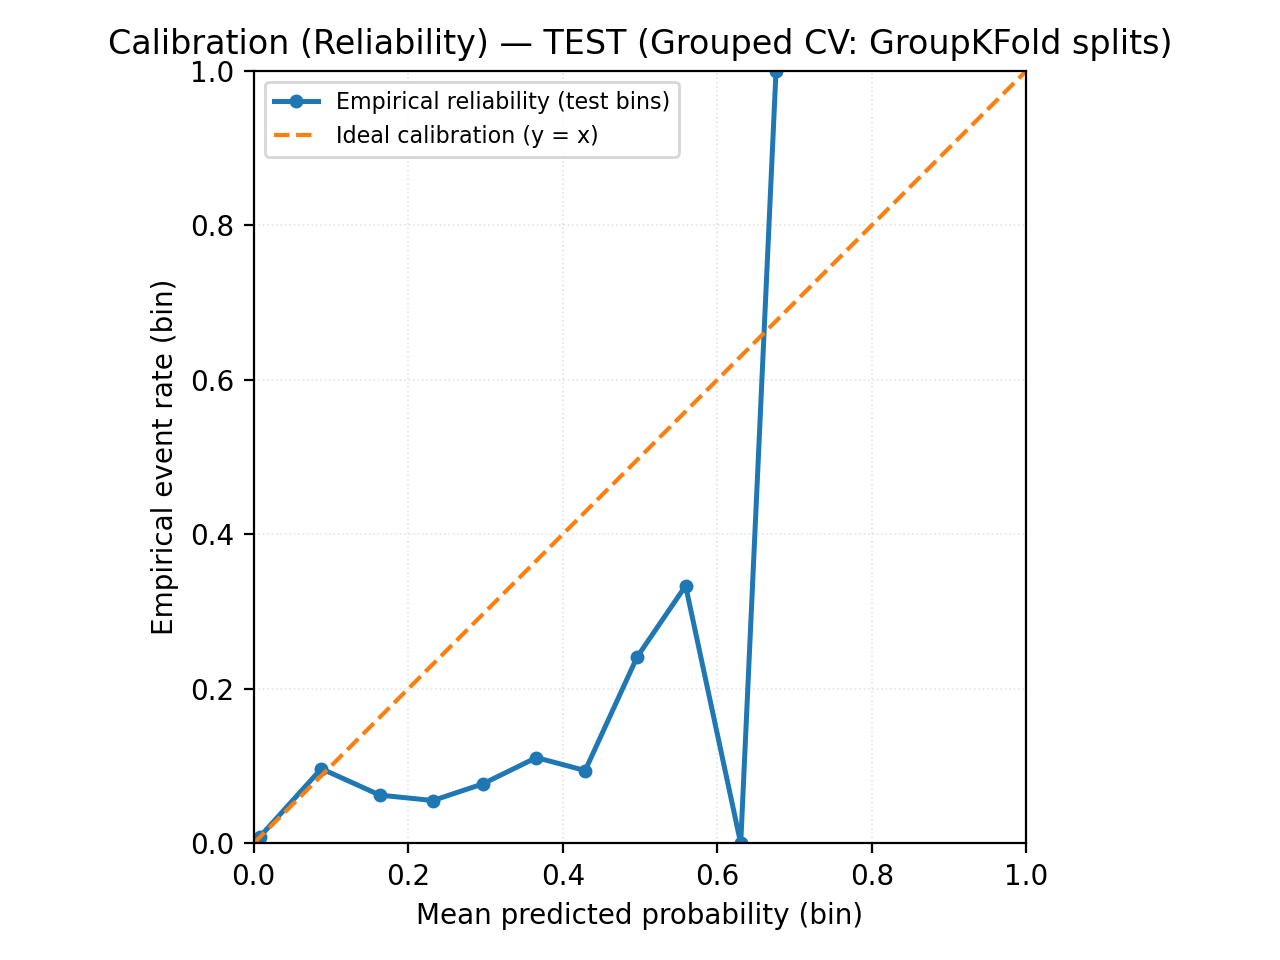
\includegraphics[width=0.45\textwidth]{outputs_v2/figures/fig_calibration_reliability_test.png}
\caption{Primary calibration evidence for weekly hazard on test rows. The figure supports the RQ1 claim only if reliability remains acceptable over operationally relevant risk bins.}
\label{fig:calibration_main}
\end{figure}

To make the right-tail reading fully auditable, Table~\ref{tab:calibration_tail_support} reports support for the highest-risk bins in the same partition used by Figure~\ref{fig:calibration_main}. The key readout is direct sample support ($n$, events, and non-events) for each tail bin.

\begin{table}[!t]
\centering
\caption{Support of the highest-risk calibration bins on test rows (same binning as Figure~\ref{fig:calibration_main}).}
\label{tab:calibration_tail_support}
\begin{tabular}{lcccc}
\hline
Bin & Risk interval & $n$ & Events & Non-events \\
\hline
Bin 8 & [0.533, 0.600) & 9 & 3 & 6 \\
Bin 9 & [0.600, 0.667) & 7 & 0 & 7 \\
Bin 10 & [0.667, 0.733) & 3 & 3 & 0 \\
\hline
\end{tabular}
\end{table}

\paragraph*{When to act: temporal decision window.}
Figure~\ref{fig:survival_baseline_rq1} connects predictive quality to decision timing. It places the baseline and policy trajectories on a common weekly axis with $T_{policy}=18$, $T_{eval\_metrics}=37$, and raw-support tail at $T_{eval\_policy}=38$. For RQ1, the baseline trajectory is the key object: periods of steeper decline define the weeks in which temporal monitoring is most decision-relevant.

\begin{figure}[!t]
\centering
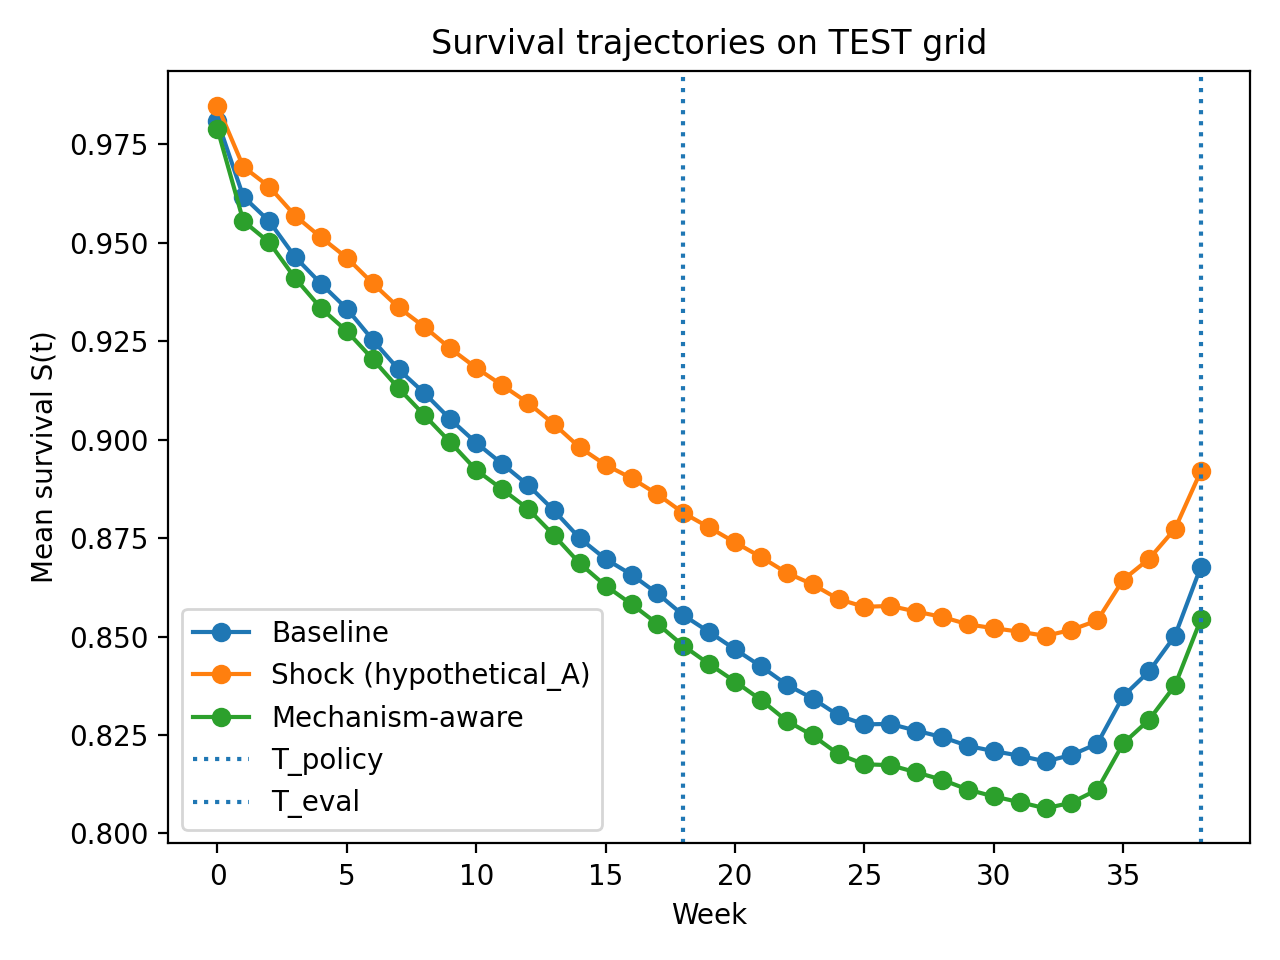
\includegraphics[width=0.45\textwidth]{outputs_v2/figures/fig_policy_survival_by_week_baseline_shock_mech.png}
\caption{Mean survival trajectories by week. For RQ1, the baseline curve is the key object: steeper decline windows indicate periods where temporal monitoring is most decision-relevant.}
\label{fig:survival_baseline_rq1}
\end{figure}

\paragraph*{RQ1 conclusion.}
Taken together, the discrimination and calibration evidence supports the intended use of the model: translating weekly risk into auditable timing signals. This conclusion, however, remains subject to the censoring-valid horizons established next.

\subsection{Censoring Validity and the Dual-Horizon Rule}
\label{subsec:censoring_results}

Before reading the RQ2 and RQ3 contrasts, the validity of the reporting horizons must be established. Figure~\ref{fig:censoring_survival_results} displays the estimated censoring survival $G(t)$ on the test set and provides the empirical justification for using two horizons rather than one.

\begin{figure}[!t]
\centering
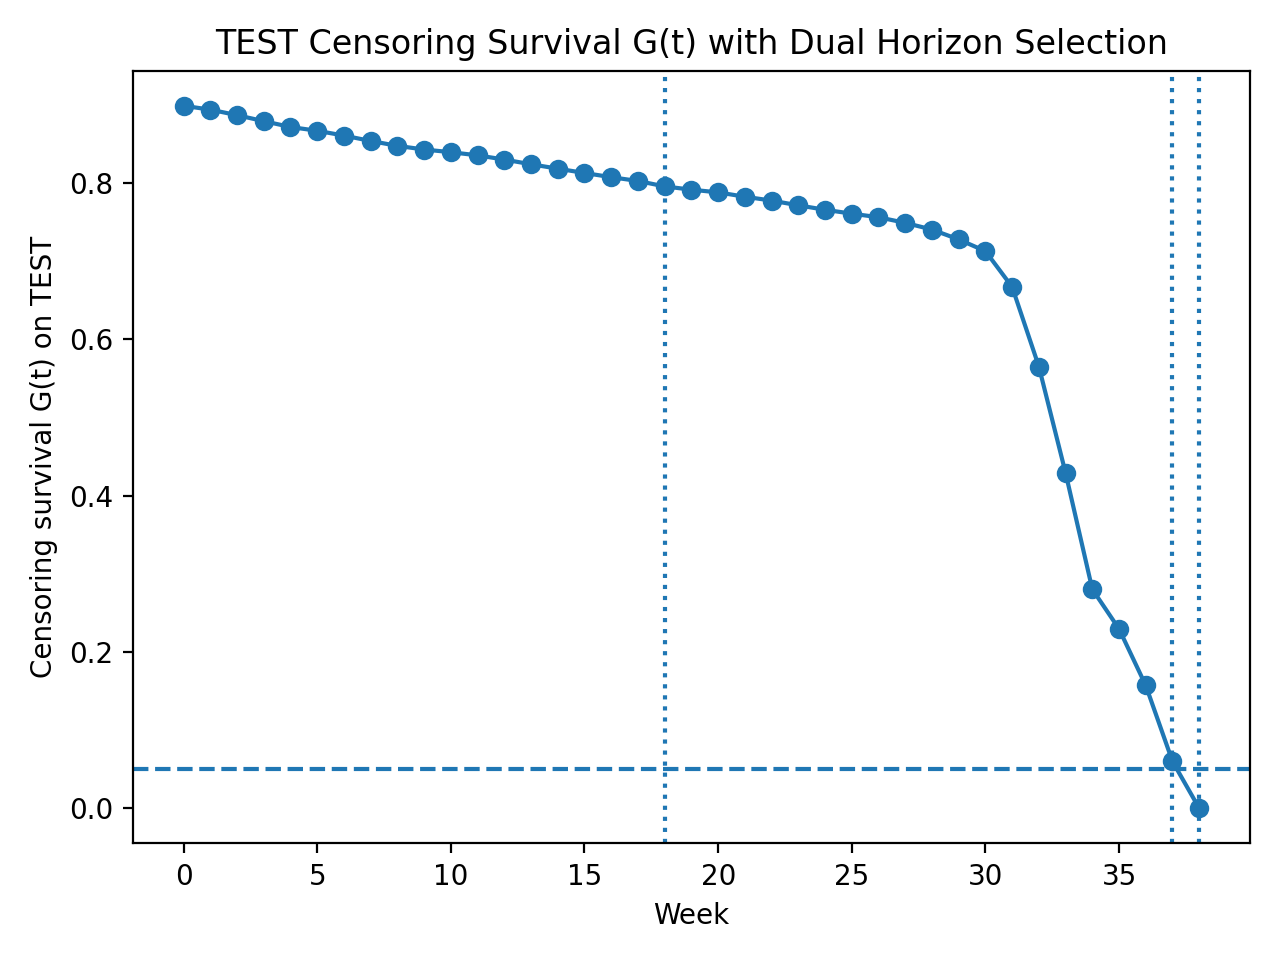
\includegraphics[width=0.45\textwidth]{outputs_v2/figures/fig_censoring_survival_G_test.png}
\caption{Censoring survival $G(t)$ used to define stable reporting horizons. The reading rule is operational: IPCW metrics are interpreted only where $G(t) \ge g_{min}=0.05$.}
\label{fig:censoring_survival_results}
\end{figure}

\begin{table}[!t]
\centering
\caption{Censoring-aware horizon diagnostics used in Results.}
\label{tab:horizon_diagnostics}
\begin{tabular}{lc}
\hline
Quantity & Value \\
\hline
$T_{policy}$ & 18 \\
$T_{eval\_metrics}$ (stable IPCW horizon) & 37 \\
$T_{eval\_policy}$ (raw support horizon) & 38 \\
$G(18)$ & 0.7958 \\
$G(37)$ & 0.0601 \\
$G(38)$ & $\approx 10^{-12}$ (unstable) \\
\hline
\end{tabular}
\end{table}

This rule is not cosmetic. It is part of the evidence contract of the section: weighted metrics and contrast summaries are interpreted only at horizons with acceptable censoring support. The distinction between $T_{policy}$, $T_{eval\_metrics}$, and $T_{eval\_policy}$ therefore determines where substantive claims are allowed to be made.

\subsection{RQ2: Policy Simulation and Structural Regime Contrast}
\label{subsec:rq2_results}

RQ2 asks whether an explicit policy rule changes model-implied survival trajectories under fixed protocol settings. The results show that the answer is yes, but the magnitude of the contrast depends strongly on how the policy enters the system.

\paragraph*{Definition used in reporting.}
\begin{equation*}
\Delta S(t)=\bar S^{(1)}(t)-\bar S^{(0)}(t),
\qquad
\bar S^{(a)}(t)=\frac{1}{N}\sum_i \hat S_i^{(a)}(t).
\end{equation*}
Positive $\Delta S(t)$ means higher survival under the policy regime than under baseline.

\paragraph*{Figure-level evidence for RQ2.}
Figure~\ref{fig:deltas_rq2} is the primary figure for RQ2. It should be read in two steps:
first, the sign over time (is the contrast above zero?);
second, the horizon-specific magnitude by scenario (what is $\Delta S$ at $T_{policy}$ and $T_{eval\_policy}$?).

\begin{figure}[!t]
\centering
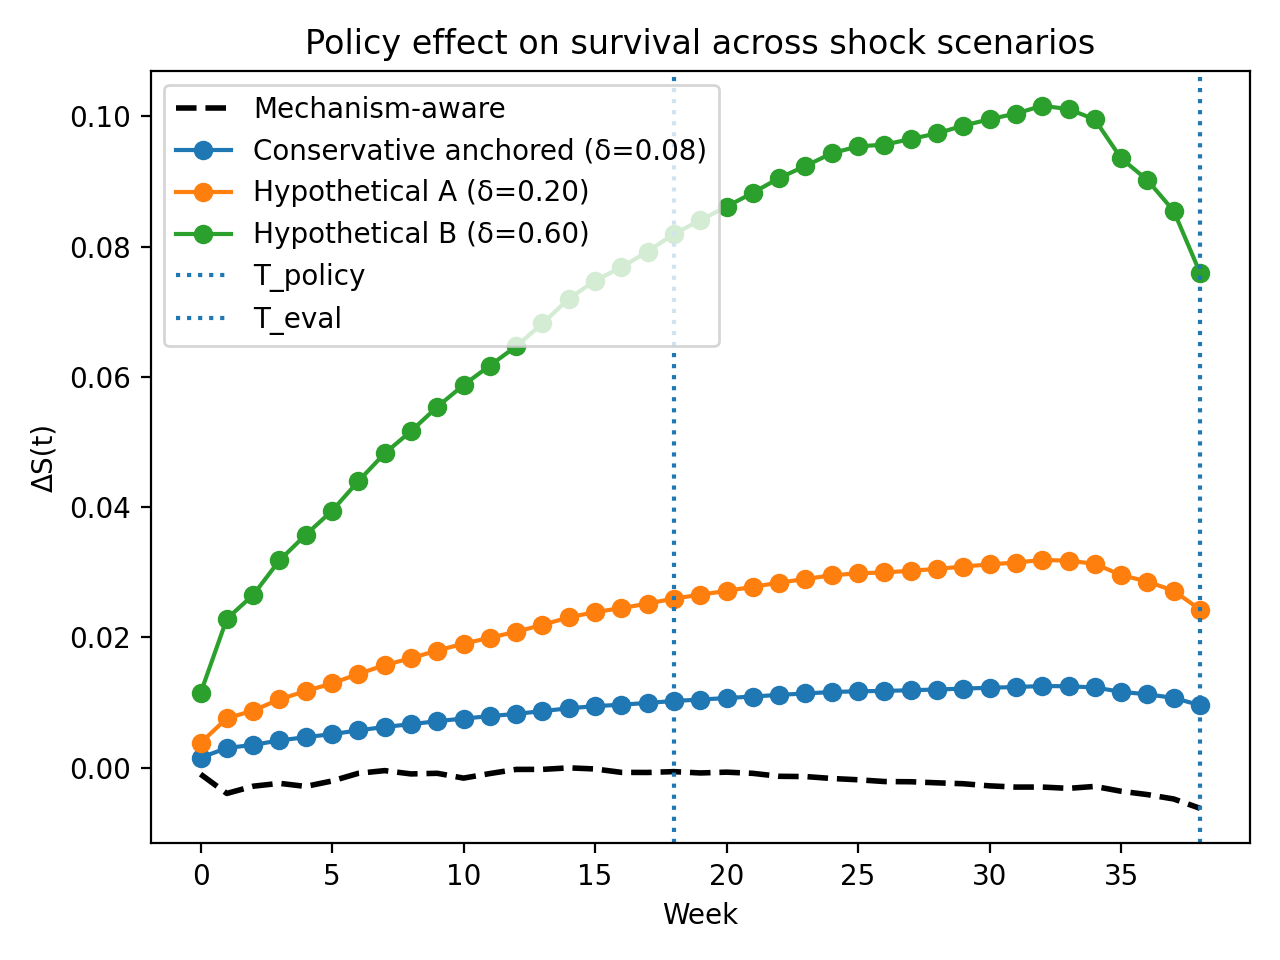
\includegraphics[width=0.45\textwidth]{outputs_v2/figures/fig_policy_deltaS_by_week_shock_scenarios.png}
\caption{Policy contrast $\Delta S(t)$ under a fixed trigger with scenario-indexed shock intensity ($\delta\in\{0.08,0.20,0.60\}$) and the shared mechanism-aware curve. The central readout is sign and horizon-specific magnitude by scenario.}
\label{fig:deltas_rq2}
\end{figure}

\begin{table}[!t]
\centering
\caption{RQ2 summary by shock-intensity scenario at $T_{policy}=18$ and $T_{eval\_policy}=38$.}
\label{tab:rq2_summary}
\small
\begin{tabular}{lcccc}
\hline
Scenario & $\delta_{shock}$ & $\Delta S_{shock}(18)$ & $\Delta S_{shock}(38)$ & $\Delta S_{mech}(18)$ \\
\hline
Anchored conservative & 0.08 & 0.0102 & 0.0096 & -0.0006 \\
Hypothetical A (reference) & 0.20 & 0.0260 & 0.0243 & -0.0006 \\
Hypothetical B (stress test) & 0.60 & 0.0819 & 0.0760 & -0.0006 \\
\hline
\end{tabular}
\end{table}

The shared mechanism-aware contrast is $\Delta S_{mech}(38)=-0.0062$ at $T_{eval\_policy}$, indicating that under the current schedule and propagated covariate channel, the mechanism-aware regime does not generate a positive survival gain in this run.

\paragraph*{Mechanism diagnostic.}
To explain why the shock and mechanism-aware regimes differ so sharply, Figure~\ref{fig:policy_mechanism_deltas} should be read as a transmission diagnostic. It shows whether policy-induced covariate deltas are large enough, and persistent enough, to alter downstream hazard meaningfully.

\begin{figure}[!t]
\centering
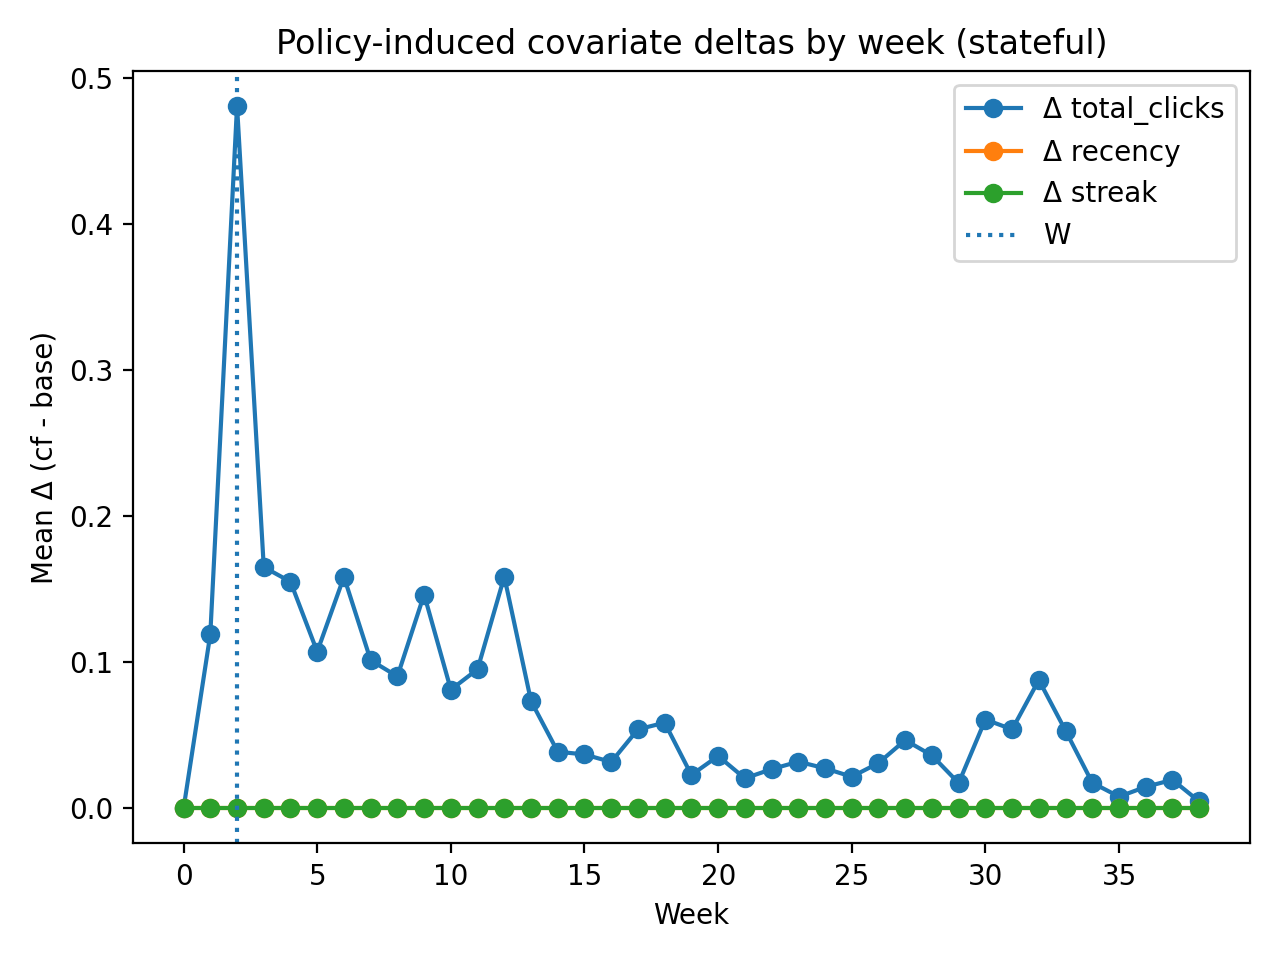
\includegraphics[width=0.45\textwidth]{outputs_v2/figures/fig_policy_covariate_deltas_by_week.png}
\caption{Mechanism diagnostic for policy propagation. Small or short-lived covariate deltas imply limited downstream hazard movement, consistent with the weak/negative mechanism-aware contrasts at fixed horizons in this run.}
\label{fig:policy_mechanism_deltas}
\end{figure}

\paragraph*{RQ2 conclusion.}
The framework answers RQ2 positively in structural terms: it can compare explicit regimes on a common temporal backbone and produce interpretable survival contrasts at fixed horizons. In the present configuration, the contrast is highly scenario-dependent in the shock branch (larger gains for larger $\delta$), while the mechanism-aware branch remains weak to negative under the current shared schedule.

\subsection{Benchmark and Robustness Evidence}
\label{subsec:benchmark_robust_results}

The purpose of this subsection is not to replace the primary track, but to test whether the main interpretation remains stable under benchmark comparison and controlled design perturbations. The benchmark families used here are the \textit{Cox time-varying benchmark} and the \textit{non-temporal enrollment-level benchmark}; together, they provide the main cross-family reference against which the primary discrete-time model is read.

\paragraph*{Cross-family benchmark.}
Figure~\ref{fig:benchmark_dual_panel} summarizes the primary model against benchmark families at aligned horizons. The key readout is directional convergence rather than rank ordering alone: the question is whether the substantive conclusion remains consistent across model families.

\begin{figure}[!t]
\centering
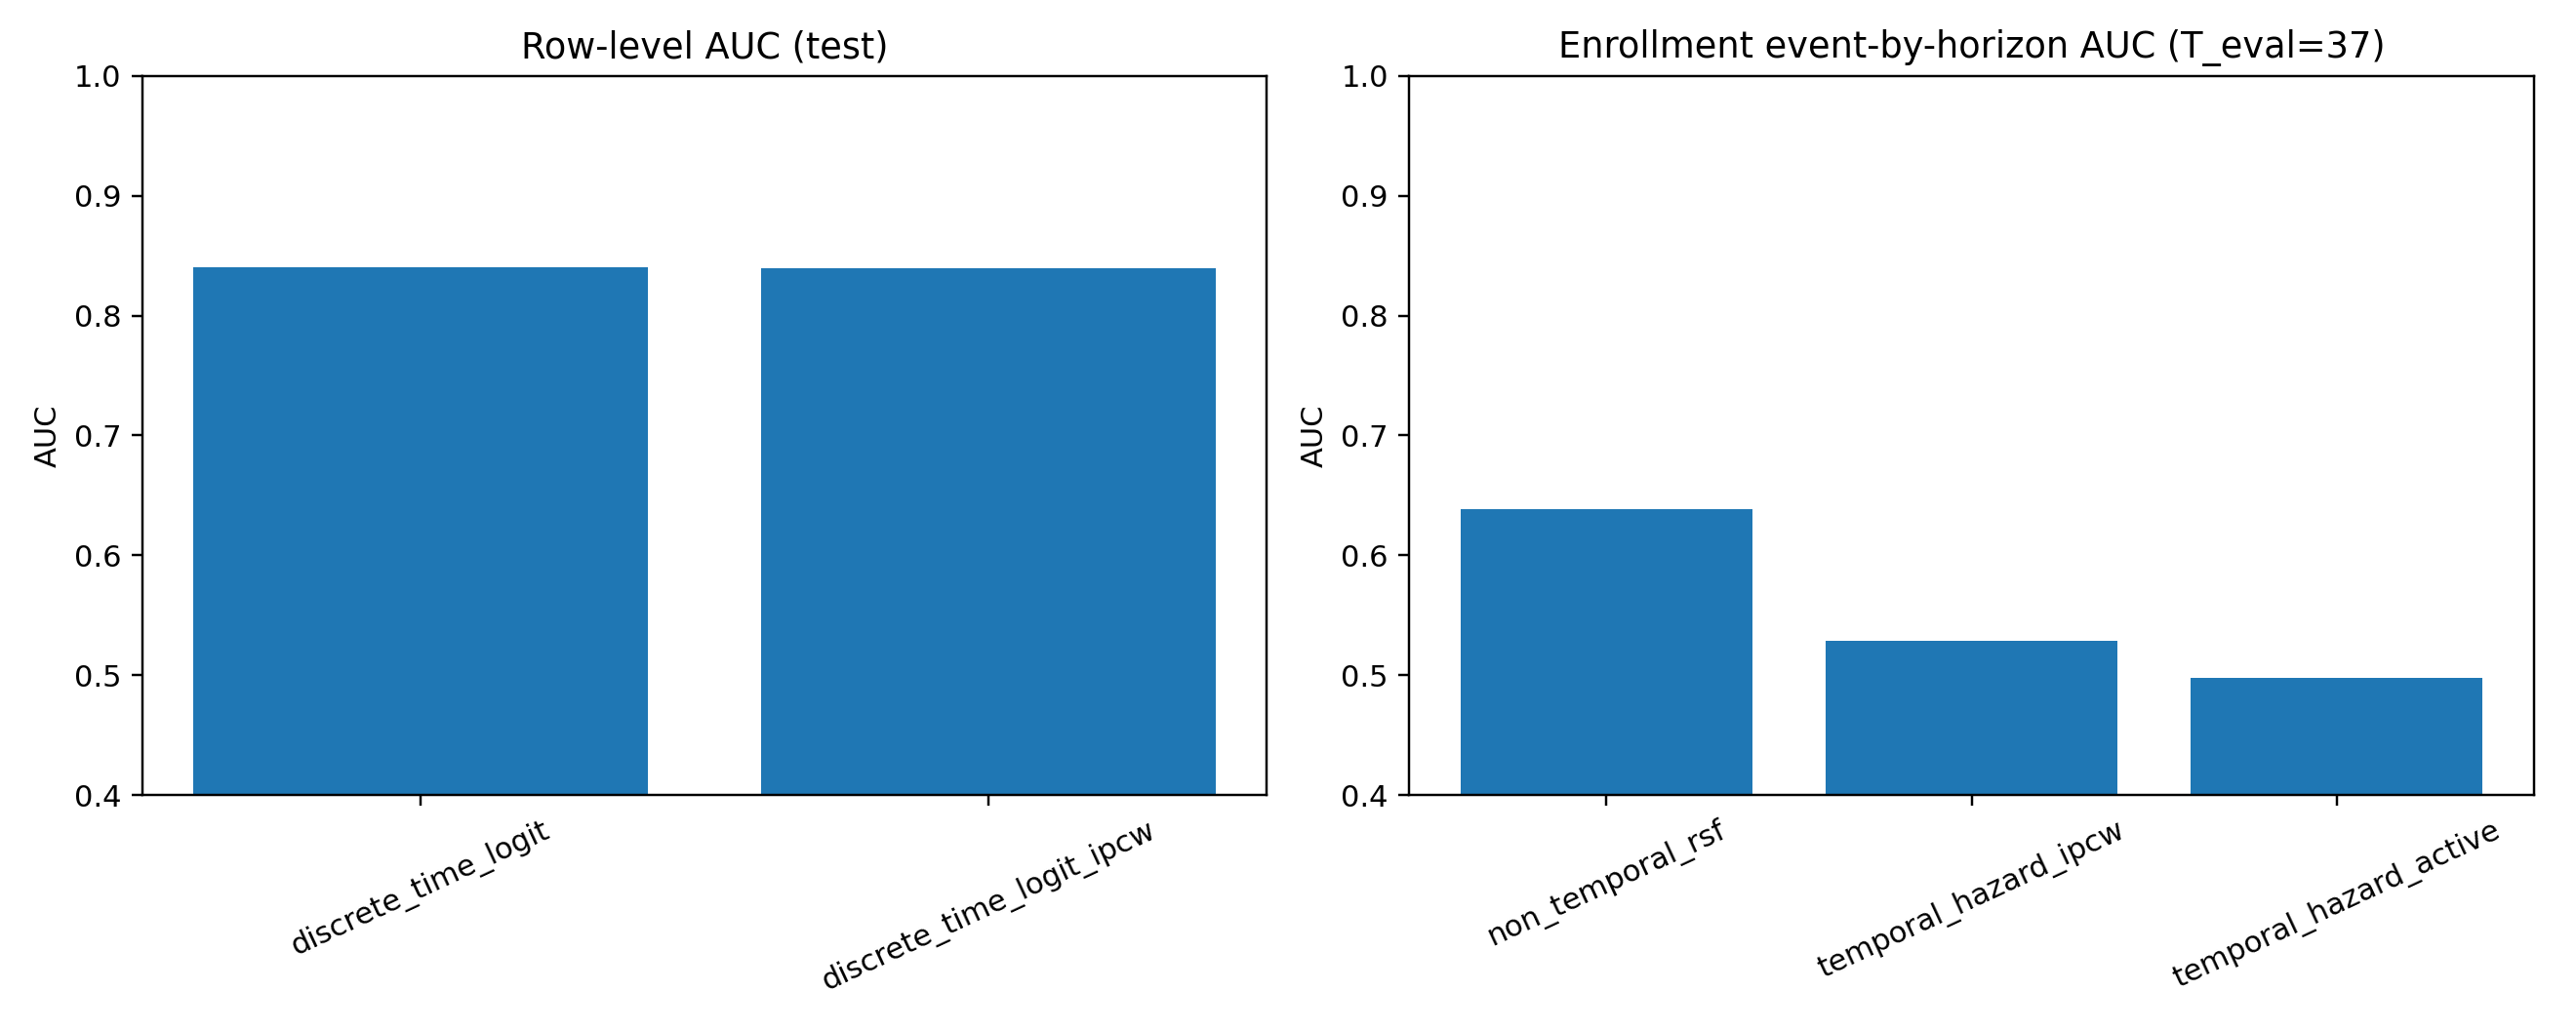
\includegraphics[width=0.45\textwidth]{outputs_v2/figures/fig_benchmark_dual_panel_auc.png}
\caption{Benchmark comparison across model families. Use this figure to verify whether the central directional conclusion is stable across the primary model, the Cox benchmark, and the non-temporal baseline.}
\label{fig:benchmark_dual_panel}
\end{figure}

\paragraph*{Ablation evidence.}
\begin{table}[!t]
\centering
\caption{Ablation at $T_{eval\_metrics}=37$ (re-trained variants).}
\label{tab:ablation_results}
\resizebox{\columnwidth}{!}{%
\begin{tabular}{lcccc}
\hline
Model & AUC$_{row,test}$ & C-index$_{discrete}$ & IPCW Brier & IPCW IBS \\
\hline
Full & 0.8396 & 0.3951 & 0.3392 & 0.1747 \\
No Recency/Streak & 0.7987 & 0.3637 & 0.3728 & 0.1772 \\
No Activity (\texttt{total\_clicks}) & 0.8263 & 0.3369 & 0.3530 & 0.1781 \\
\hline
\end{tabular}%
}
\end{table}

Removing Recency/Streak causes the largest AUC drop, which is consistent with the proposed role of temporal regularity features in supporting weekly hazard quality.

\paragraph*{Endpoint sensitivity.}
\begin{table}[!t]
\centering
\caption{Endpoint sensitivity at $T_{eval\_metrics}=37$.}
\label{tab:endpoint_sensitivity_results}
\resizebox{\columnwidth}{!}{%
\begin{tabular}{lcc}
\hline
Metric & Primary (Withdrawn) & Composite (Fail OR Withdrawn) \\
\hline
C-index$_{discrete}(T_{eval\_metrics})$ & 0.4965 & 0.4965 \\
IPCW Brier($T_{eval\_metrics}$) & 0.8542 & 1.0799 \\
IPCW IBS($0..T_{eval\_metrics}$) & 0.2429 & 0.3291 \\
$N_{events}$ & 2{,}216 & 4{,}308 \\
\hline
\end{tabular}%
}
\end{table}

The directional reading is preserved, while calibration and risk quality shift under endpoint broadening. This is the intended role of this robustness axis: to show where the conclusion is stable and where metric quality changes under alternative endpoint definitions.

\paragraph*{Out-of-domain generalization.}
\begin{table}[!t]
\centering
\caption{Held-out run generalization (five runs).}
\label{tab:ood_results_short}
\small
\resizebox{\columnwidth}{!}{%
\begin{tabular}{lrrrrr}
\hline
Held-out run & Rows & Pos. rate & AUC$_{row}$ & Enrollments & Events \\
\hline
\texttt{CCC-2014J} & 57{,}760 & 0.0145 & 0.7652 & 2{,}498 & 836 \\
\texttt{FFF-2014J} & 56{,}546 & 0.0112 & 0.8393 & 2{,}365 & 636 \\
\texttt{BBB-2014J} & 52{,}440 & 0.0095 & 0.7934 & 2{,}292 & 497 \\
\texttt{FFF-2013J} & 57{,}054 & 0.0088 & 0.8317 & 2{,}283 & 504 \\
\texttt{BBB-2013J} & 52{,}849 & 0.0078 & 0.8381 & 2{,}237 & 410 \\
\hline
\end{tabular}%
}
\end{table}

AUC variability across held-out runs reveals course-run heterogeneity. This limits direct portability across settings, but it does not invalidate the framework itself; rather, it identifies the scale at which domain sensitivity should be expected.

\subsection{RQ3: Subgroup Validation via Change-in-Gap}
\label{subsec:rq3_results}

RQ3 tests whether the same policy regime produces differential group contrasts, reported with uncertainty. The emphasis here is not on a broad fairness claim, but on whether the framework can quantify subgroup-sensitive structural contrasts on the same simulation backbone used for aggregate policy evaluation.

\paragraph*{Reported quantity.}
\begin{equation*}
\Delta Gap(T)=Gap^{(1)}(T)-Gap^{(0)}(T).
\end{equation*}
Negative values indicate reduced gap under policy relative to baseline for the group coding used in this run.

\paragraph*{Primary figure-level evidence.}
The fairness interpretation pipeline is summarized in Figure~\ref{fig:fairness_pipeline_graph}. Figures~\ref{fig:rq3_gap_tpolicy} and \ref{fig:rq3_gap_teval} are then read as horizon-specific outputs of that pipeline.

\begin{figure}[!t]
\centering
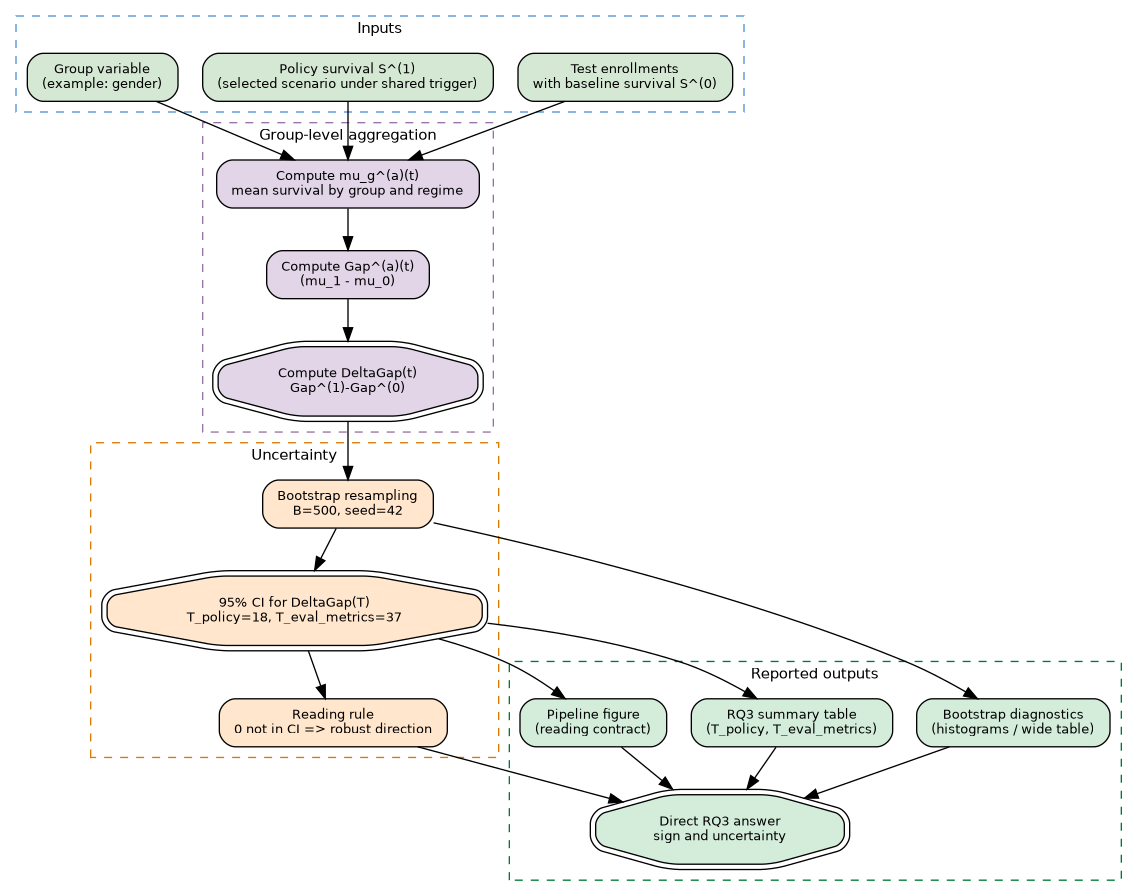
\includegraphics[width=0.45\textwidth]{figures/fig_fairness_pipeline.png}
\caption{Fairness/subgroup pipeline used in RQ3. It links groupwise survival aggregation, change-in-gap computation, and bootstrap uncertainty for a selected policy scenario under the shared trigger contract.}
\label{fig:fairness_pipeline_graph}
\end{figure}

\begin{figure}[!t]
\centering
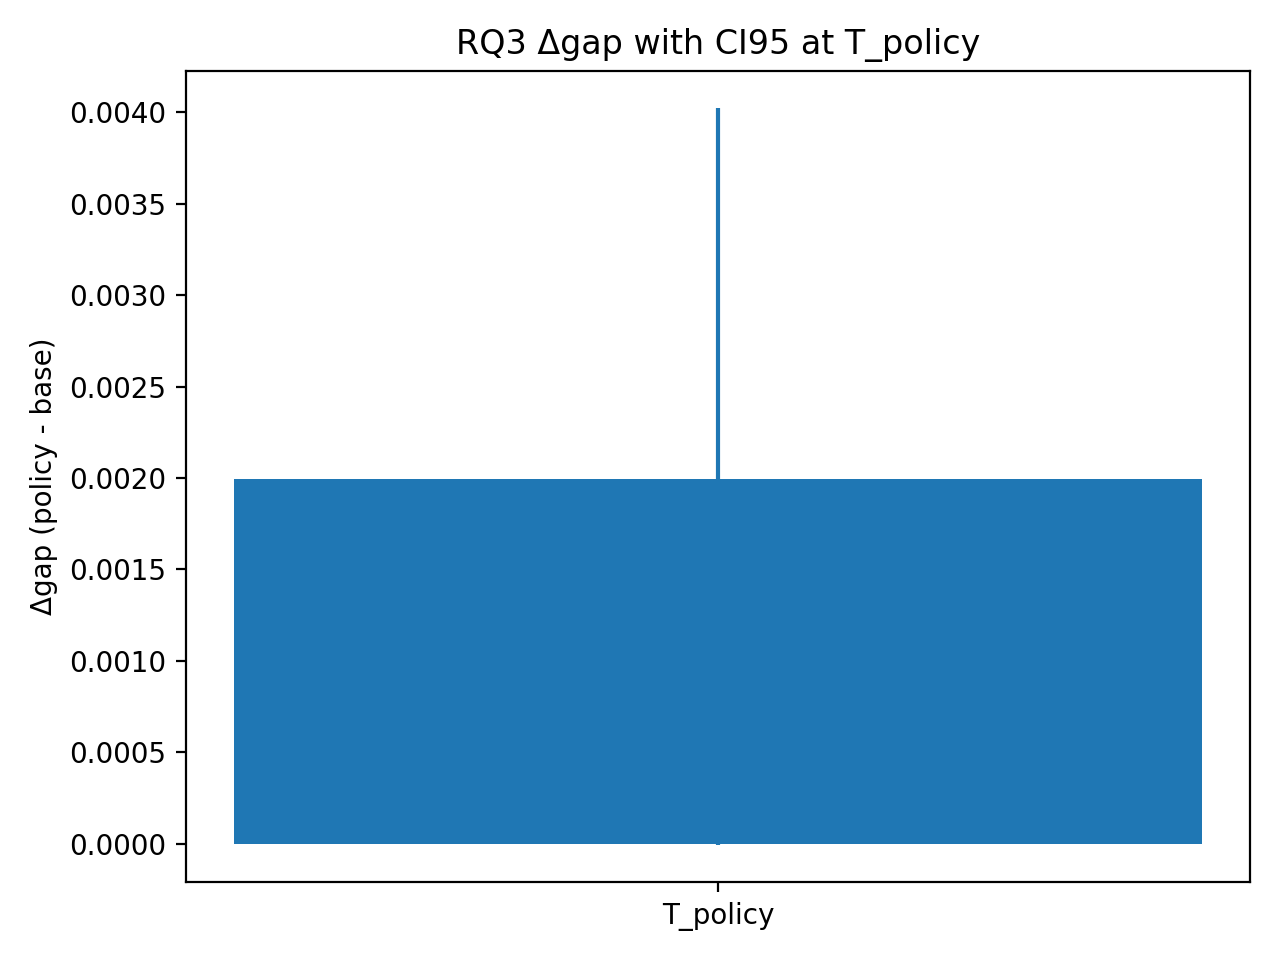
\includegraphics[width=0.45\textwidth]{outputs_v2/figures/fig_rq3_gap_Tpolicy.png}
\caption{RQ3 gap result at $T_{policy}=18$. Interpretation requires combining sign, magnitude, and confidence-interval support.}
\label{fig:rq3_gap_tpolicy}
\end{figure}

\begin{figure}[!t]
\centering
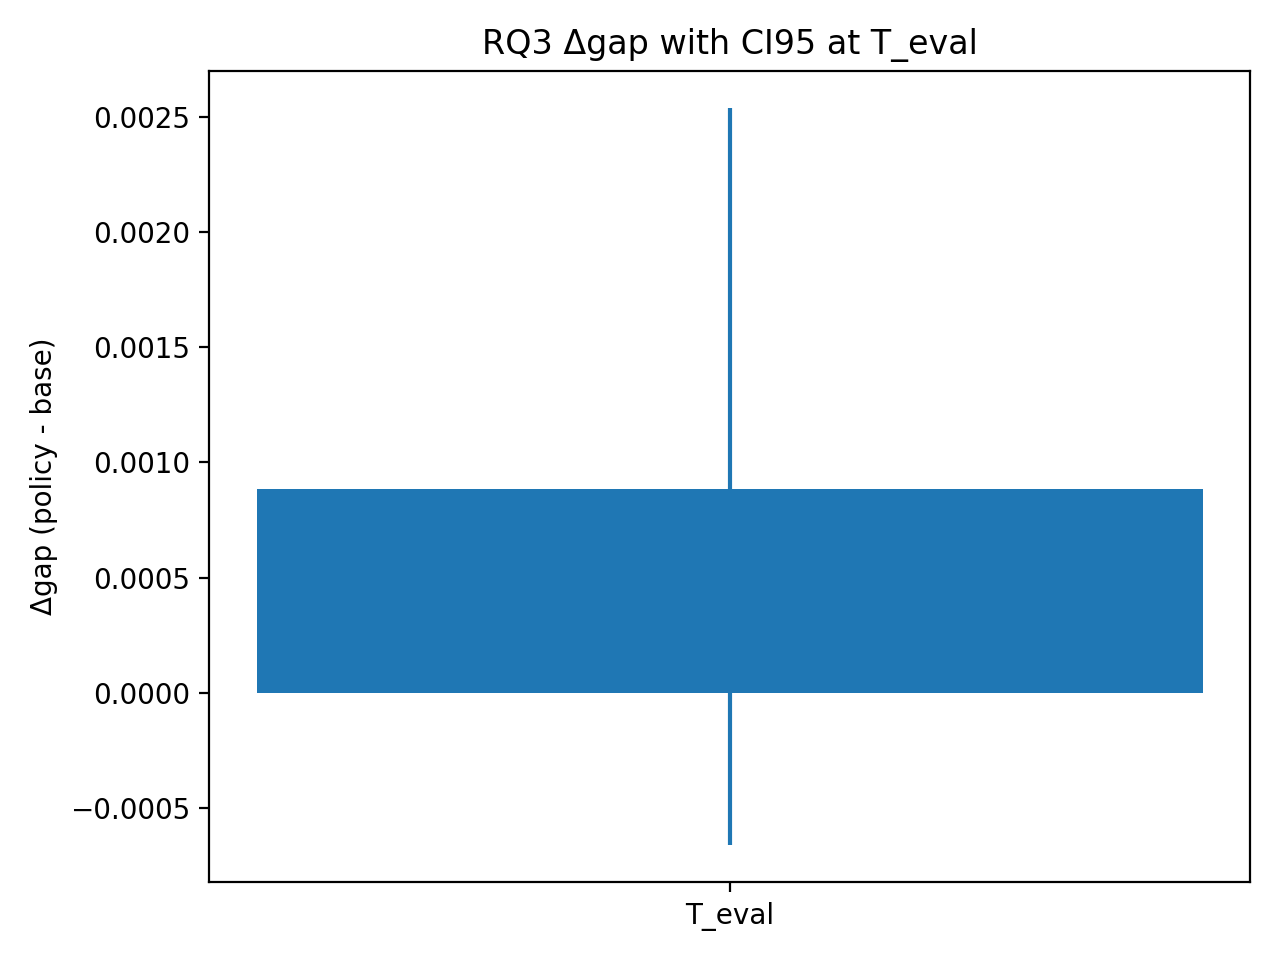
\includegraphics[width=0.45\textwidth]{outputs_v2/figures/fig_rq3_gap_Teval.png}
\caption{RQ3 gap result at $T_{eval\_metrics}=37$. Consistency with $T_{policy}$ is part of the robustness readout.}
\label{fig:rq3_gap_teval}
\end{figure}

\begin{table}[!t]
\centering
\caption{RQ3 summary with bootstrap uncertainty.}
\label{tab:rq3_summary}
\begin{tabular}{lcc}
\hline
Horizon & $\Delta Gap(T)$ & 95\% bootstrap CI \\
\hline
$T_{policy}=18$ & $-0.00050816$ & $(-0.00066222,\,-0.00032944)$ \\
$T_{eval\_metrics}=37$ & $-0.00056691$ & $(-0.00071529,\,-0.00040728)$ \\
\hline
\end{tabular}
\end{table}

Both intervals exclude zero, so the direction is robust at both horizons for the reported scenario.

\paragraph*{RQ3 conclusion.}
The framework answers RQ3 positively at the level it proposes: it can quantify subgroup-sensitive structural contrasts and attach uncertainty to their directional interpretation. This supports the use of the subgroup track as an auditable extension of the policy-simulation framework rather than as a separate fairness model.

\subsection{Results Synthesis: What the Paper Set Out to Answer}
\label{subsec:results_synthesis}

The paper set out to move from static prediction---who is at risk---to a temporal, decision-oriented framework that addresses when to act and how to compare explicit regimes. The empirical evidence supports that objective in four direct points:

\begin{enumerate}
\item Weekly hazard quality is sufficient for temporal decision support (RQ1).
\item Regime comparison is operational and auditable through $\Delta S(t)$ (RQ2).
\item The same policy can be audited for subgroup differentials via $\Delta Gap(T)$ (RQ3).
\item The main interpretation remains directionally coherent under benchmark and robustness axes.
\end{enumerate}

These are framework-validation claims under explicit scenario rules. They are not causal claims about real interventions in OULAD.

\subsection{Interpretation Boundaries}

To prevent overclaim, the results are interpreted under three explicit limits:
\begin{itemize}
\item policy and fairness outputs are simulated regime contrasts;
\item horizon-validity constraints under censoring are binding for metric interpretation;
\item endpoint and domain-shift robustness indicate sensitivity ranges, not universal transportability.
\end{itemize}

Within these limits, the section answers the paper objective directly: a reproducible temporal pipeline can translate weekly risk into explicit, auditable policy and subgroup diagnostics.